\chapter{Trigger Scouting System Luminosity}


\section{BIB monitoring with EMTF++}

Another potential use of the scouting data will be for monitoring of high radius beam-induced backgrounds.
As described in section~\ref{sec:Chapter5:BIBTheory}, these particles may arise from the interaction of the beam with the collimators or beam gas far from CMS and arrive with trajectories aproximately parallel to the beam at high radius.
For Phase-2, the upgraded Endcap Muon Track Finder algorithm (EMTF++) is designed to reconstruct transversly displaced muons \cite{CERN-LHCC-2020-004}.
Displaced muons reconstruced by the EMTF++ would be sent the GMT together with the normal endcap muon list.
These L1 muon candidates may be selected from the GMT muons and  counted similarly to the BMTF muons.
This measurement will provide an additional beam quality flag in real time, redundant to the BHM system.
In the studies presented in \cite{CERN-LHCC-2020-004}, the efficiency for detecting displaced muons with the EMTF++ was approxmately 50\% and constant as a function of the transerverse displament ($d_0$), however the muon sample used for those studies only covered $d_0<$1.2 m.
At the time of writing, further studies are underway including beam halo simulation to understand the efficiency of the reconstruction algorithm for tracks with angles parallel to the beam and at higher radius.


%%Displaced muon track reco at EMTF
%%Muon list sent to GMT
%%GMT List sent to Scouting
%%Select tags and histogram at Scouting
%%Send to BRILDAQ along with BMTF, EMTF, OMTF
%%
%%TDR-021 Page 97: displaced muons
%%- d0 < 120 cm
%%- 1.2 < |eta| <2.4
%%- |z0| < 30 cm
%%
%%BHM from BRIL TDR:
%%- r=180 - 190 cm  
%%- distancefrom the IP of z = 2000 - 2030 cm

\begin{figure}[hbtp]
\centering
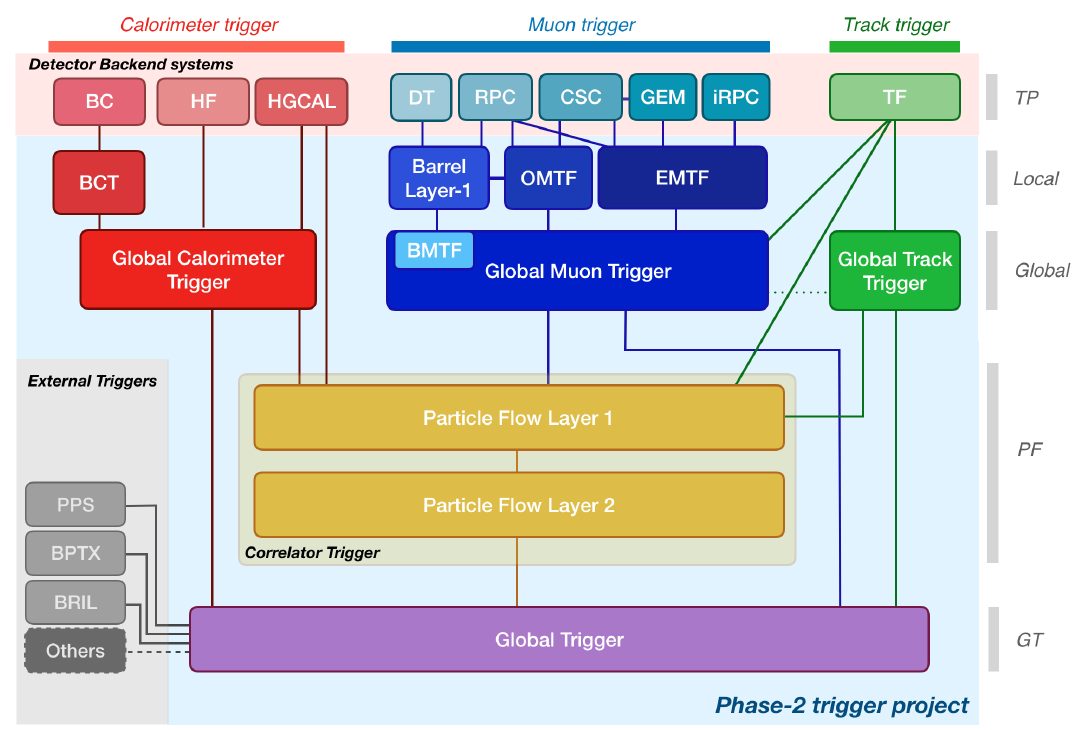
\includegraphics[width=.7\linewidth]{tex/Part2/fig/Phase2TriggerProject-TDR021-Page8.png}
\caption{
Design of the Phase-2 Trigger Project [TDR-021].
}
\label{fig:Phase2TriggerProject}
\end{figure}

\begin{figure}[hbtp]
\centering
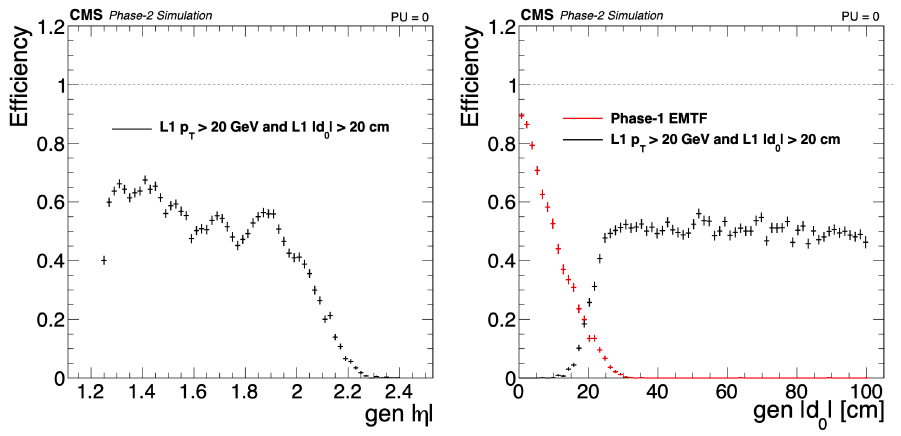
\includegraphics[width=.97\linewidth]{tex/Part2/fig/EMTFpp_eff_vs_eta_d0.png}
\caption{
EMTF++ displaced muon efficiency [TDR-021].
}
\label{fig:Phase2TriggerProject}
\end{figure}

\begin{figure}[hbtp]
\centering
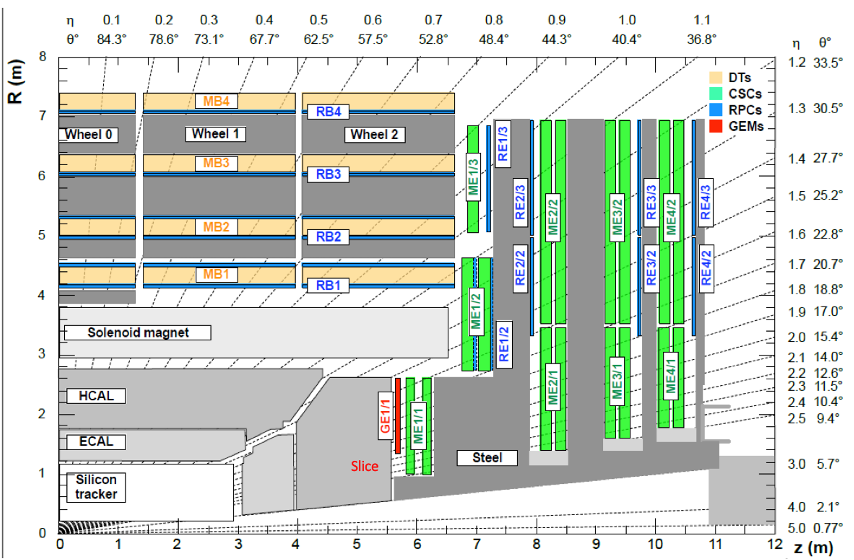
\includegraphics[width=.7\linewidth]{tex/Part2/fig/DT-longitudinal.png}
\caption{
Muon system layout.
}
\label{fig:MuonSystem}
\end{figure}





